\documentclass{beamer}

\begin{document}
\begin{frame}
  \frametitle{(Integer) Linear Models}
  \begin{columns}
    \column{0.6\textwidth}
    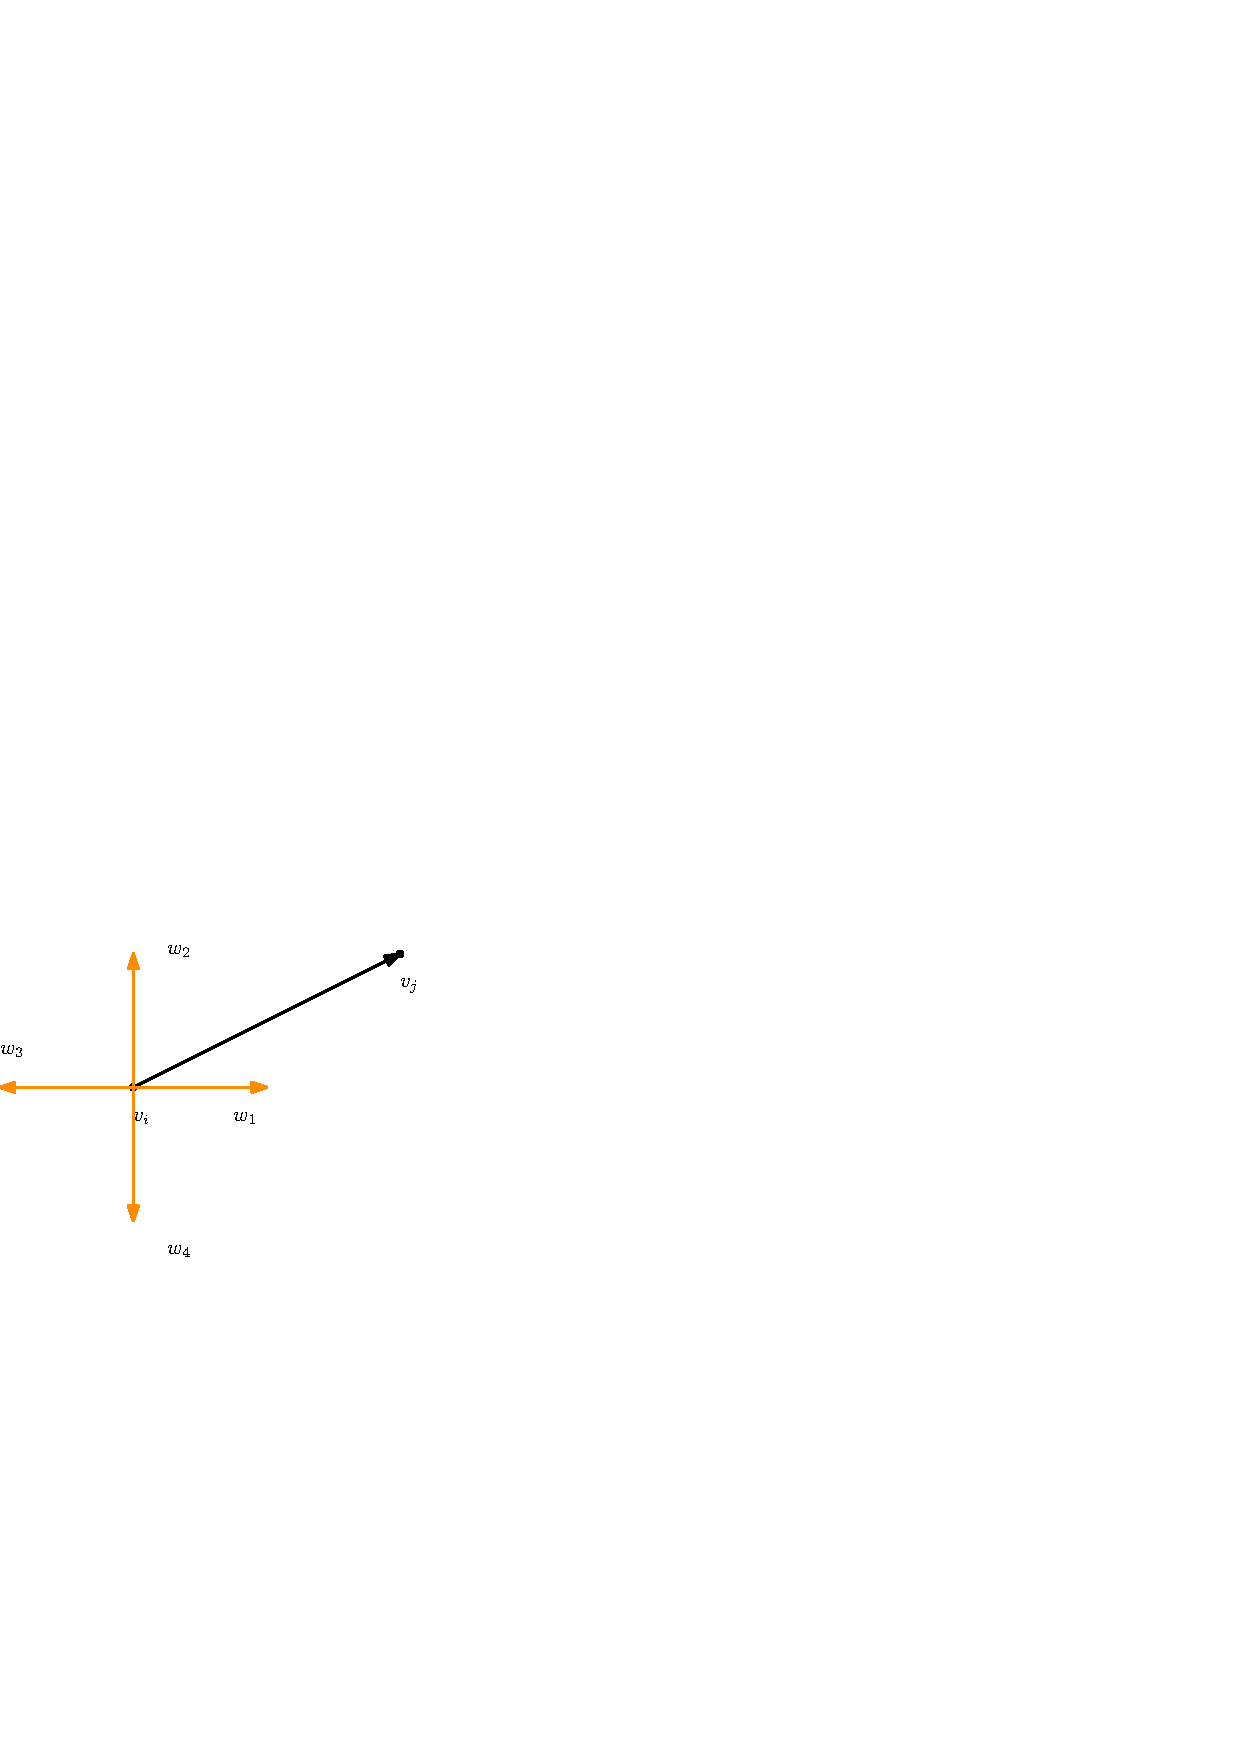
\includegraphics[width=\columnwidth]{snapping.pdf}
    \column{0.4\textwidth}
    \begin{align*}
      \min \sum_{(i,j) \in E} |\epsilon_{i,j,1}| +& |\epsilon_{i,j,2}| \\
      \tilde{v}_i + \ell_{i,j}\sum_{d\in 1\dots 4}c_{i,j,d}w_d &= v_j+\epsilon_{i,j}\\
      c_{i,j,d} &\in \{0, 1\}\\
      \sum_{d} c_{i,j,d} &= 1\\
      \ell_{i,j} &= \| v_i - v_j\|
    \end{align*}
  \end{columns}

\end{frame}

\begin{frame}
  \frametitle{Linear Models}
  \begin{columns}
    \column{0.6\textwidth}
    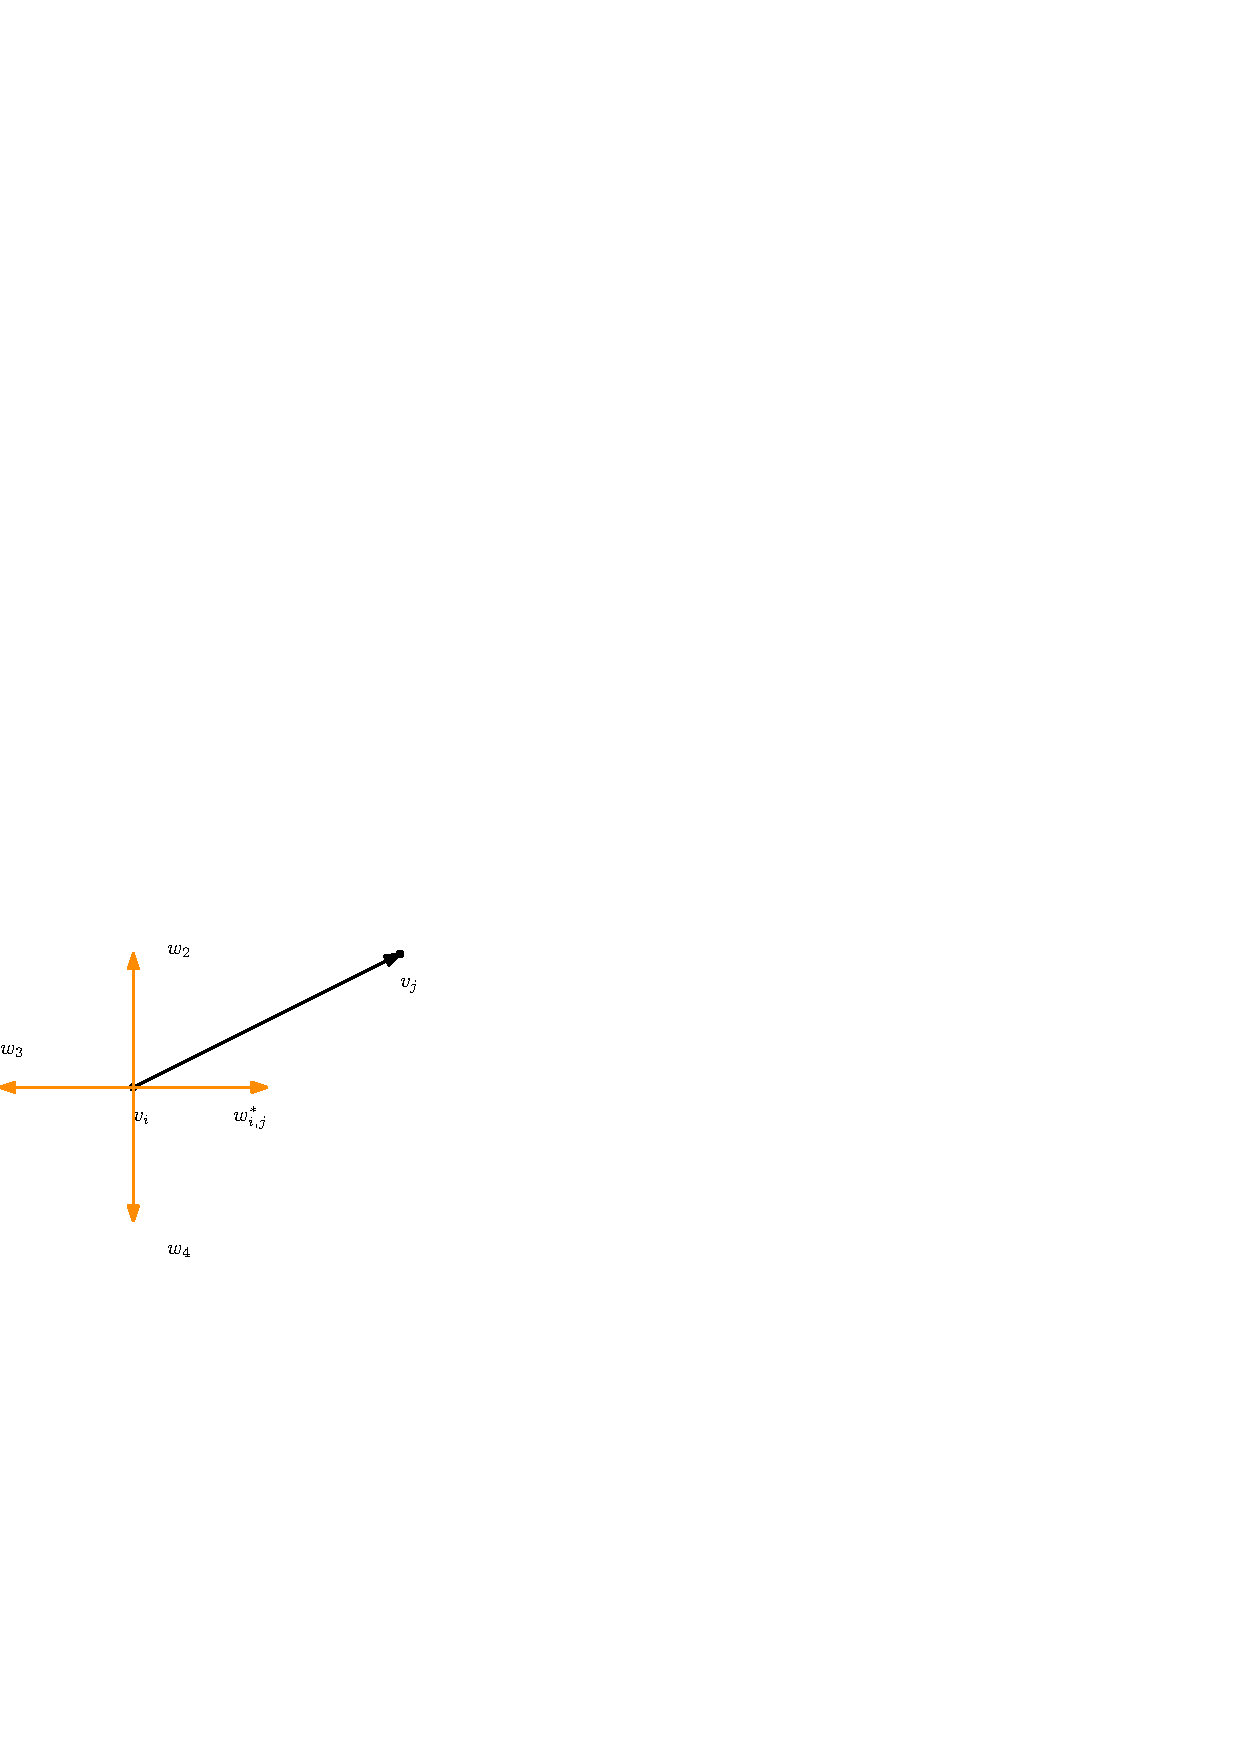
\includegraphics[width=\columnwidth]{snapping2.pdf}
    \column{0.4\textwidth}
    \begin{align*}
       \max \sum_{(i,j) \in E} \langle z_{i,j} &, w^*_{i,j} \rangle\\
      z_{i,j} & = (\tilde{v}_{i} - \tilde{v}_{j})/l_{i,j}\\
       w^*_{i,j}&= \text{closest $w_d$}\\
       \ell_{i,j} &= \| v_i - v_j\|
    \end{align*}
    In both cases we need penalties/bounds to prevent vertices from
    moving too far.
  \end{columns}
\end{frame}

\end{document}
